\chapter{Introducción}


\section{Motivación y antecedentes}

Dada la gran expansión de Internet desde los años 90, la seguridad se ha convertido en algo 
fundamental. Hoy en día el uso de Internet se ha generalizado, llegando a todas las áreas, 
desde finanzas hasta el envío de pruebas médicas, pasando por compras, redes sociales y demás, 
por lo que la seguridad es algo primordial. 
\intro De esta forma llegamos al emparejamiento de flujos, el cual es muy útil para los NMS, 
sistemas de monitoreo de red, \textit{Network Monitoring System}, como podría ser BRO \cite{broindex}.
Gracias al uso de estos programas el administrador de sistemas podrá prevenir ataques, como por ejemplo, los 
de denegación de servicio, DDoS, \textit{Distributed Denial of Service}. Un administrador de sistemas deberá de 
garantizar que el recurso que facilita y gestiona esté operativo siempre, por lo tanto deberá de analizar el 
tráfico para evitar los posibles ataques, virus, etc.


\intro Existen otras técnicas de clasificación de tráfico, como se puede ver en el artículo del 
departamento \citep{comparacion}, estas técnicas son: 

\begin{itemize}
\item Clasificación basada en los puertos de la capa de transporte. \cite{iana}
\item Clasificación basada en el contenido del paquete. \cite{payload}
\item Clasificación basada en la aplicación de técnicas de aprendizaje automático sobre estadísticas de tráfico. \cite{learning}
\end{itemize}
Estas técnicas no son muy eficaces hoy en día, pues por ejemplo, la primera de las tres puede ser burlada 
haciendo pasar cualquier tipo de conexión por el puerto 80. La segunda bastará con que los datos estén 
encriptados para que no se pueda acceder al paquete, a parte de que no respeta la privacidad. Por lo tanto estas 
dos técnicas son obviadas y se utiliza la tercera como opción más fiable, aunque tiene como inconveniente que 
necesita tiempo para aprender a clasificar bien el tráfico.

\intro Por lo tanto es necesario un nuevo método de clasificación, que sea funcional en cualquier circunstancia 
y sea eficiente desde el principio. Por lo tanto el método de emparejamiento planteado por el departamento es 
muy atractivo al ser necesario saber solo las IP's y los puertos. \cite{comparacion}

\section{Objetivos}

El objetivo del trabajo es desarrollar un módulo para Bro. En este módulo irá implementada la técnica de emparejamiento de flujos, de forma que pueda ser usada en redes fuera de un entorno de laboratorio.

\intro Para ello será necesario conocer como Bro gestiona los flujo, desde su nacimiento a su muerte. 
\intro También hará falta gestionar las entradas y salidas, aunque al principio se hará uso de un 
archivo \textit{pcap} de prueba para controlar si todo funciona bien, 
pudiendo pasar luego a analizar el tráfico de una red online.
\intro Será necesario controlar Bro de una forma eficiente, dado que se gestiona desde la linea de comandos 
podemos hacer que Bro no haga uso de los módulos.


\section{Metodología}

Para realizar este trabajo se establecen una serie de tareas:

\begin{itemize}
\item Familiarización con Bro.
\item Pruebas con el lenguaje propio de Bro.
\item Lectura del artículo del departamento. \cite{comparacion}
\item Desarrollo del módulo en Bro.
\item Pruebas del módulo.
\end{itemize}


FALTA DIAGRAMA DE GANTT.

\intro Este proyecto no necesita de ningún gasto, pues Bro \cite{broindex} proporciona sus binarios de 
forma gratuita. El módulo será subido a GitHub con licencia de software libre, por lo que cualquiera 
podrá usarlo o modificarlo en el futuro. El único gasto es el de un ordenador con Linux, o bien con Mac OS, 
pues de momento no está disponible para Windows. \cite{brodownload}


\section{Estructura de la memoria}

Esta memoria se organizará de la siguiente forma: En el capítulo 2 se hablará de 
todos los fundamentos teóricos y tecnológicos sobre los que se basa este proyecto. 
En el capítulo 3 se contará cómo se pretende resolver el problema expuesto. En el 
capítulo 4 se encontrarán detalles de cómo se han implementado los diferentes módulos. 
En el capítulo 5 se verán las pruebas realizadas, para comprobar que todo funciona como 
estaba previsto, tanto a nivel funcional, como a nivel de aplicación. En el último capítulo 
se verán las conclusiones del trabajo y cómo podría seguir trabajándose en el futuro.



\section{Capas de Red}

Como ya sabrá, Internet sigue un modelo capas y que hay varios modelos para 
organizar estas capas, como el TCP/IP y el OSI \cite{redes2010}.

\begin{figure}[H]
  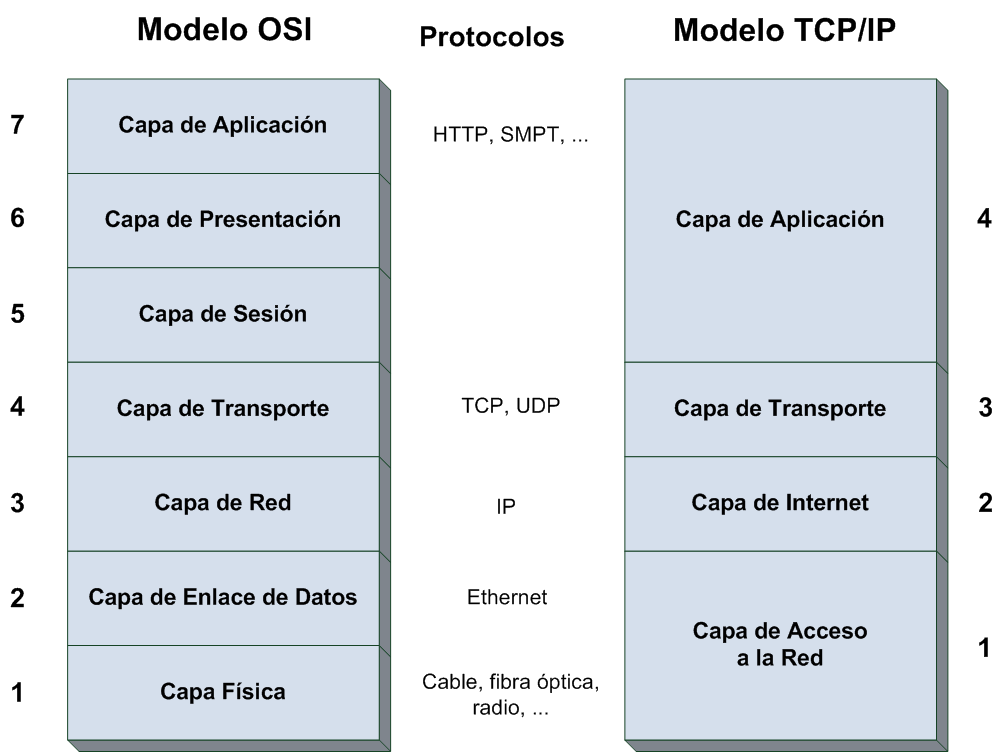
\includegraphics[width=1\textwidth]{imagenes/capas.png}
  \centering
  \caption{Modelos de capas de Internet.}
\end{figure}

\noindent Nosotros seguiremos el \textit{modelo TCP/IP}, y a continuación, procederemos a dar 
unas pinceladas sobre la capa de aplicación, la de transporte y la de enlace.

\subsection{Capa de aplicación}

En la capa de aplicación encontramos las aplicaciones de red y sus protocolos. 
Los protocolos que encontramos en esta capa son \textbf{HTTP, SMTP y FTP}. 
\intro
\begin{itemize}
\item El protocolo \textit{HTTP} permite la solicitud y transferencia de documentos web.
\item El protocolo \textit{SMTP} permite la transferencia de mensajes de correo electrónico.
\item El protocolo \textit{FTP} permite la transferencia de archivos entre dos terminales.
\end{itemize}

\noindent A parte de estos protocolos también corresponde a esta capa el \textbf{DNS}, 
que es el encargado de traducir los nombres de los sitios web.

\subsection{Capa de transporte}

La capa de transporte es la encargada de transportar los mensajes de la capa de aplicación. 
Los protocolos de esta capa son \textbf{TCP y UDP}. La principal diferencia y será algo que 
marque el trabajo es que \textit{TCP} está orientado a garantizar la conexión, mientras que \textit{UDP} no 
garantiza la conexión.

\subsection{Capa de red}

En la capa de red es donde nos encontramos el protocolo \textbf{IP} y también 
un protocolo, \textbf{ICMP}, que nuestro \textit{NMS} hay veces que localiza y 
sitúa junto con \textit{TCP y UDP}, aunque no pertenezca a la capa de transporte.
\intro
En esencia, esta capa es la que se encarga de transportar los \textit{datagramas} 
de un \textit{host} a otro.

\subsection{¿Qué es útil para nosotros?}

En nuestro caso nos quedaremos solamente en la capa de transporte, 
ignorando la información que podamos obtener de la capa 
de aplicación. En caso de que nuestro NMS lo detecte, incluiremos ICMP, 
pero solo para añadir más 
información a los distintos flujos que podemos llegar a analizar, 
pero despreciaremos la información relativa al resto de esta capa. 
El archivo pcap que utilizaremos para la prueba será \textit{nitroba.pcap}, 
el cual se puede obtener desde la web de Bro y el cual se corresponde con 
la obtención del tráfico de una universidad de Sudáfrica.
